\documentclass{article}
\usepackage[T1]{fontenc}
\usepackage{lmodern}
\usepackage{amssymb,amsmath}
\usepackage{ifxetex,ifluatex}
\usepackage{unicode-math}
\usepackage{booktabs}
\usepackage{minted}
\usepackage{float}
\usepackage{listings}
\usepackage{cite}
\usepackage{tikz}
\usepackage{mathpartir}
\usepackage[toc,page]{appendix}
\usepackage{xspace}
\usepackage{pdfpages}
\usepackage{lastpage}
\usepackage{fancyhdr}
\usepackage{verbatim}
\usepackage[a4paper,left=4cm,right=4cm,top=3cm,bottom=2.5cm]{geometry}
% use upquote if available, for straight quotes in verbatim environments
\IfFileExists{upquote.sty}{\usepackage{upquote}}{}
\usepackage{xltxtra,xunicode}
\defaultfontfeatures{Mapping=tex-text,Scale=MatchLowercase}
\setmonofont[Mapping=tex-ansi]{DejaVu Sans Mono}
% \setmainfont{Times New Roman}
% use microtype if available
\IfFileExists{microtype.sty}{\usepackage{microtype}}{}

\usepackage{graphicx}
% Redefine \includegraphics so that, unless explicit options are
% given, the image width will not exceed the width of the page.
% Images get their normal width if they fit onto the page, but
% are scaled down if they would overflow the margins.
\makeatletter
\def\ScaleIfNeeded{%
  \ifdim\Gin@nat@width>\linewidth
    \linewidth
  \else
    \Gin@nat@width
  \fi
}
\makeatother
\let\Oldincludegraphics\includegraphics
{%
 \catcode`\@=11\relax%
 \gdef\includegraphics{\@ifnextchar[{\Oldincludegraphics}{\Oldincludegraphics[width=\ScaleIfNeeded]}}%
}%
\ifxetex
  \usepackage[setpagesize=false, % page size defined by xetex
              unicode=false, % unicode breaks when used with xetex
              xetex]{hyperref}
\else
  \usepackage[unicode=true]{hyperref}
\fi
\hypersetup{breaklinks=true,
            pdfauthor={Adam Schønemann and Oscar Toro},
            pdftitle={Fingertrees in Coq},
            colorlinks=true,
            citecolor=blue,
            urlcolor=blue,
            linkcolor=magenta,
            pdfborder={0 0 0}}
\urlstyle{same}  % don't use monospace font for urls
\setlength{\parindent}{0pt}
\setlength{\parskip}{6pt plus 2pt minus 1pt}
\setlength{\emergencystretch}{3em}  % prevent overfull lines
\setcounter{secnumdepth}{5}

\newcommand{\code}[1]{\texttt{#1}}

\lhead{Fingertrees in Coq}
\rhead{PLS, ITU Spring 2017}
\cfoot{Page \thepage\ of \pageref{LastPage}}

\title{Fingertrees in Coq}

\author{Adam Schønemann\\ \code{adsc@itu.dk} \and Oscar Felipe Toro \\ \code{osto@itu.dk}}
\date{}

\begin{document}
\pagenumbering{gobble}
% 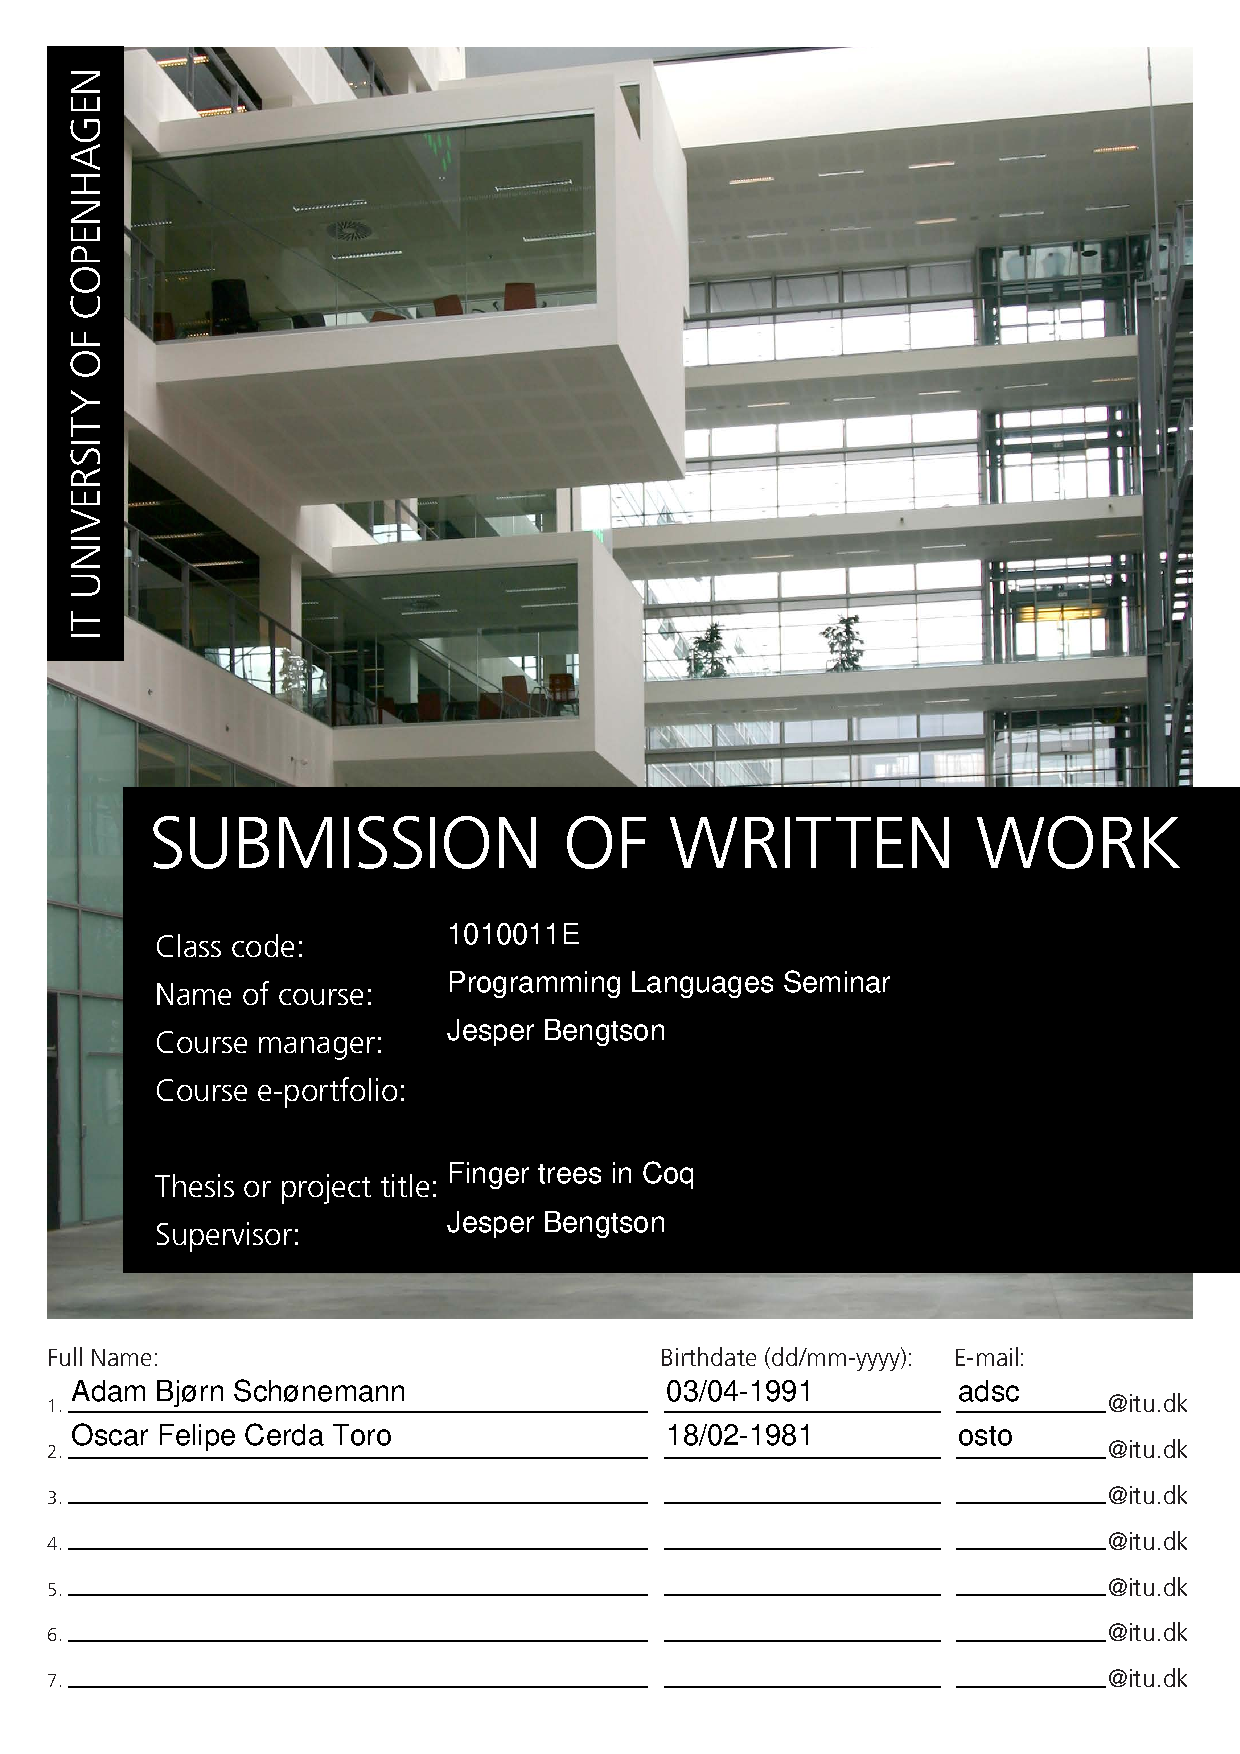
\includepdf{imgs/frontpage.pdf}
\pagenumbering{arabic}
\tableofcontents
\pagestyle{fancy}
\maketitle
\thispagestyle{fancy}
\section{Introduction}
This report is a project hand-in for the ``Programming Languages Seminar'' class at
the IT University of Copenhagen.
It describes a verified implementation of finger trees in Coq, derived from
Hinzes and Paterson's paper on finger trees in Haskell\cite{Hinze-Paterson:FingerTree}.

\section{Finger trees}
A finger tree is a functional and persistent data-structure that represents a sequence.
First published by Leonidas J. Guibas in 1977\cite{guibas1977new},
and later refined to 2-3 finger trees in Haskell \cite{Hinze-Paterson:FingerTree},
it is used today in many libraries, most notably Haskell's \code{Data.Sequence}
module in the standard library.

Finger trees allow amortized constant time pushing and popping from both ends of the
sequence, as well as an amortized logarithmic time append and split operations.
Finger trees can also be adapted to work as random-access sequences or priority queues.

\subsection{Definition}
A finger tree is in many ways like a 2-3 tree, that is, a tree where all nodes have
either 2 or 3 children, and all data is contained in the leaves. However, finger trees
extend the 2-3 tree with ``fingers'' - that is, a 2-3 tree with a prefix and a suffix ``finger''. A finger is typically represented by a ``digit'' which is a buffer of
elements stored left to right. This leads us to the final definition of a finger tree:

\textbf{A finger tree is either:}
\begin{itemize}
\item An empty finger tree
\item A finger tree containing a single element of type $A$, or
\item A finger tree containing a prefix digit with elements of type $A$, a deeper finger tree containing elements of of type $\textsf{node } A$, and a suffix digit with
elements of type $A$
\end{itemize}

where \textsf{node} is a 2-3 node. This leads us directly to the following definition in Coq:

\begin{listing}[H]
\begin{minted}[linenos]{coq}
(** A node contains two or three values of A*)
Inductive node (A:Type) : Type :=
| node2: A -> A -> node A
| node3: A -> A -> A -> node A.

(** Digits hold one to four elements of A *)
Inductive digit (A:Type) : Type :=
| one : A -> digit A
| two : A -> A -> digit A
| three : A -> A -> A -> digit A
| four : A -> A -> A -> A -> digit A.

(** A fingertree is either empty, a single thing, or a deeper fingertree
    along with a prefix digit and a suffix digit *)
Inductive fingertree (A:Type) : Type :=
| empty : fingertree A
| single : A -> fingertree A
| deep : digit A -> fingertree (node A) -> digit A -> fingertree A.
\end{minted}
\end{listing}
Listing \ref{ft_ex_01} shows a tree representation of a sequence, and
figure \ref{ft-viz} shows a visualization of this structure. Note that
for one sequence, there can be many fingertree representations. The definition
of \code{fingertree} is a so-called \textit{non-regular} or \textit{nested}
datatype. This is because in its inductive parameter, its type variable $A$
is instantiated with a new type (namely $\textsf{node } A$). This type
encodes that at each deeper level of a tree, its digits contain further nested
nodes of $A$. However, this nested definition forces all recursive definitions
on \code{fingertree}s to use polymorphic recursion -- later we shall see that
this will make proofs on \code{fingertree}s considerably harder in Coq.

\begin{listing}[H]
\begin{minted}[linenos]{coq}
Example ft_ex_01 : fingertree nat :=
  deep (two 1 2)
       (deep (two (node2 3 4) (node2 5 6))
             empty
             (two (node3 7 8 9) (node2 10 11))
       )
       (three 12 13 14).
\end{minted}
\caption{A \code{fingertree} encoding of the sequence $\{1,2,\dots,14\}$.}
\label{ft_ex_01}
\end{listing}

\begin{figure}[H]
\centering
\begin{tikzpicture}
  [scale=.8,auto=left,every node/.style={circle,draw}, y=-1.5cm, x=1.5cm]
  \node [scale=0.5] (j11) at (4.5,0) {};
  \node [scale=0.5] (j12) at (5.5,0) {};
  \node [scale=0.5] (j21) at (4.8,2) {};
  \node [scale=0.5] (j22) at (5.2,2) {};
  \node [scale=0.5] (j31) at (1.5,4) {};
  \node [scale=0.5] (j32) at (3.5,4) {};
  \node [scale=0.5] (j33) at (5,4) {};
  \node [scale=0.5] (j34) at (7,4) {};
  \node [scale=0.5] (j35) at (9.5,4) {};

  \node (n21)  at (2,2) {1};
  \node (n22)  at (3,2) {2};
  \node (n23)  at (7,2) {12};
  \node (n24)  at (8,2) {13};
  \node (n25)  at (9,2) {14};
  \node (n41)  at (1,6) {3};
  \node (n42)  at (2,6) {4};
  \node (n43)  at (3,6) {5};
  \node (n44)  at (4,6) {6};
  \node (n45)  at (6,6) {7};
  \node (n46)  at (7,6) {8};
  \node (n47)  at (8,6) {9};
  \node (n48)  at (9,6) {10};
  \node (n49)  at (10,6) {11};

  % first level junctions
  \draw (j11) -- (j21);
  \draw (j12) -- (j22);

  % first level junctions to nodes
  \draw (j11) -- (n21);
  \draw (j11) -- (n22);
  \draw (j12) -- (n23);
  \draw (j12) -- (n24);
  \draw (j12) -- (n25);

  % second lvl junctions (1)
  \draw (j21) -- (j31);
  \draw (j21) -- (j32);
  \draw (j21) -- (j33);

  % second lvl junctions (2)
  \draw (j22) -- (j33);
  \draw (j22) -- (j34);
  \draw (j22) -- (j35);

  % third lvl junctions to nodes
  \draw (j31) -- (n41);
  \draw (j31) -- (n42);
  \draw (j32) -- (n43);
  \draw (j32) -- (n44);
  \draw (j34) -- (n45);
  \draw (j34) -- (n46);
  \draw (j34) -- (n47);
  \draw (j35) -- (n48);
  \draw (j35) -- (n49);
\end{tikzpicture}
\caption{A visualization of the fingertree representation in listing \ref{ft_ex_01}.}
\label{ft-viz}
\end{figure}


\subsection{Reducable}
To capture the fact that a finger tree represents a sequence, we must define
how to convert between a tree and a sequence. As functional programmers, we
of course love lists, so the sequence we'll be focusing on is the list. That is,
we want to define two definitions

\begin{minted}{coq}
Definition to_list {A : Type} (tr : fingertree A) : list A.
Definition to_tree {A:Type} (s: list A) : fingertree A .
\end{minted}

However, we can actually be far more general than this, by generalizing a sequence
to ``something that can be folded over''. Another word for fold is ``reduce'', so
we shall use this term in the spirit of \cite{Hinze-Paterson:FingerTree}.
Thus, we define the type-class \code{reduce} as:

\begin{minted}{coq}
Class reduce F := Reduce {
  reducer : forall {A} {B}, (A -> B -> B) -> (F A -> B -> B);
  reducel : forall {A} {B}, (B -> A -> B) -> (B -> F A -> B);
}.
\end{minted}

A type constructor \code{F} that implements \code{reduce} can be reduced from the
right or the left by giving it a reducing function and an initial accumulator.

Both \code{node} and \code{digit} are type constructors that represent sequences,
and can thus be folded over as such:

\begin{listing}[H]
\begin{minted}[linenos]{coq}
Instance node_reduce : reduce node :=
  {|
    reducer :=  fun A B op nd z =>
                match nd with
                | node2 a b => op a (op b z)
                | node3 a b c => op a (op b (op c z))
                end;

    reducel :=  fun A B op z nd =>
                match nd with
                | node2 b a => op (op z b) a
                | node3 c b a => op (op (op z c) b) a
                end;
  |}.

Instance digit_reduce : reduce digit :=
  {|
    reducer :=  fun A B op dg z =>
                match dg with
                | one a => op a z
                | two a b => op a (op b z)
                | three a b c => op a (op b (op c z))
                | four a b c d => op a (op b (op c (op d z)))
                end;

    reducel :=  fun A B op z db =>
                match dg with
                | one a => op z a
                | two b a => op (op z b) a
                | three c b a => op (op (op z c) b) a
                | four d c b a => op (op (op (op z d) c) b) a
                end;
  |}.
\end{minted}
\end{listing}

We can now also make \code{fingertree} and instance of \code{reduce} as such:

\begin{listing}[H]
\begin{minted}[linenos]{coq}
Instance fingertree_reduce : reduce fingertree :=
  {|
    reducer :=  fix ft_reducer {A} {B} op tr z :=
                match tr with
                | empty => z
                | single x => op x z
                | deep pr m sf =>
                  let op' := reducer op in
                  let op'' := ft_reducer (reducer op) in
                  op' pr (op'' m (op' sf z))
                end;

    reducel :=  fix ft_reducel {A} {B} op z tr :=
                match tr with
                | empty => z
                | single x => op z x
                | deep pr m sf =>
                  let op'  := reducel op in
                  let op'' := ft_reducel (reducel op) in
                  op' (op'' (op' z pr) m) sf
                end;
  |}.
\end{minted}
\caption{Instancing \code{fingertree} as \code{reduce}.}
\label{ft_reduce}
\end{listing}

Note again that the definitions in \ref{ft_reduce} make use of polymorphic
recursion.

We can now easily define \code{to\_list} for any reducible, including \code{fingertree}s.

\begin{minted}[linenos]{coq}
Definition to_list {F: Type -> Type} {r: reduce F} {A : Type} (s : F A) : list A :=
  reducer cons s nil.
\end{minted}

To go the other way around, i.e. \code{to\_tree} we can use the same trick, however
we must first define an equivalent operation to \code{cons} on trees. That is,
an operation that can add an $A$ to a $\textsf{fingertree} A$.

\subsection{Adding to trees}
Since finger trees are designed to be efficient deques, we can add to both the
left and right of the finger tree. We shall go through the implementation
of the left add operation only -- the right add is similar.

First, consider a tree such as \code{deep (one 2) empty (one 3)}. We can easily
add a number to the left of this tree, simply by exchanging the left prefix
\code{one 2} by \code{two 1 2}. The same strategy works when the prefix is
constructed with either \code{one}, \code{two} or \code{three}. Also, in
base cases where the tree is \code{empty} or \code{single} are also trivial.
However, if the prefix is constructed with \code{four},
then we cannot simply add a value to the digit.
We shall have to shuffle the deeper tree around to make room
for the new value in the top-most prefix. Recursion helps us here -- we can
simply choose to insert the tthree right-most values of the prefix into the
deeper tree, and recursion will make sure they're inserted at the first position
where there is ``room'' for them. The resulting definition in Coq is thus:

\begin{listing}[H]
\begin{minted}[linenos]{coq}
(** Add to the left of a fingertree *)
Fixpoint addl {A:Type} (a:A) (tr:fingertree A) : fingertree A :=
  match tr with
  | empty                    => single a
  | single b                 => deep (one a) empty (one b)
  | deep (one b)        m sf => deep (two a b) m sf
  | deep (two b c)      m sf => deep (three a b c) m sf
  | deep (three b c d)  m sf => deep (four a b c d) m sf
  | deep (four b c d e) m sf => deep (two a b) (addl (node3 c d e) m) sf
  end.
\end{minted}
\end{listing}

Using \code{addl} we can now define \code{to\_tree} as

\begin{minted}{coq}
Definition to_tree {F:Type -> Type} {A:Type} {r:reduce F} (s:F A) :
  fingertree A := reducer addl s empty.
\end{minted}

\subsection{Viewing trees}
Another aspect in capturing the sequence represented by a finger tree is to deconstruct
the tree as the conjunction of a an $A$ and a (possibly empty) $\textsf{fingertree} A$.
We can call this a ``view'' of the tree. Finger trees can be viewed from both
the left and right side. We shall only elaborate on the left side -- the right
side view is implemented similarly.

We shall define a new data structure that represents the view as
\begin{minted}{coq}
Inductive View_l (S:Type -> Type) (A:Type): Type :=
| nil_l : View_l S A
| cons_l : A -> S A -> View_l S A.
\end{minted}

Notice that \textit{a)} it closely mirrors how a list is deconstructed, and
\textit{b)} it is generalized over all type constructors.

To construct a \code{View\_l} from a \code{fingertree} we must define a function
\code{view\_l}.
We get a similar (albeit reversed) situation to the definition of \code{addl}
above -- viewing base cases and trees with prefixes greater than one is
trivial, but in the case of \code{deep (one x) m sf} we have to reshuffle
the deeper tree, since we cannot have empty digits.

Consider the value \code{deep (one x) m sf} of type \code{fingertree A}. Then,
\code{m} must have type \code{fingertree (node A)}.
If we want to view it from the left, we should get \code{cons\_l x m'} where
\code{m' : fingertree A}. Thus, we must somehow ``flatten'' \code{m}.
We can view \code{m} recursively and pattern match on it.
\begin{enumerate}
  \item if \code{view\_l m = nil\_l} we must construct a \code{fingertree A} out
        of the suffix \code{sf : digit A}. Since \code{digit} implements \code{reduce},
        we can simply call \code{to\_tree sf}.
  \item if \code{view\_l m = cons\_l a m'}, then \code{a : node A} and
        \code{m' : fingertree (node A)}. We can then construct our new fingertree
        using the \code{deep} constructor,
        by converting \code{a} to a \code{digit A} and using \code{m'} and \code{sf}
        as the deeper tree and suffix respectively.
\end{enumerate}

Thus, we get the following Coq definition for \code{view\_l}:

\begin{listing}[H]
\begin{minted}[linenos]{coq}
Fixpoint view_l {A:Type} (tr:fingertree A) : View_l fingertree A :=
  match tr with
  | empty                    => nil_l
  | single x                 => cons_l x empty
  | deep (four x y z u) m sf => cons_l x (deep (three x y u) m sf)
  | deep (three x y z)  m sf => cons_l x (deep (two x y) m sf)
  | deep (two x y)      m sf => cons_l x (deep (one x) m sf)
  | deep (one x)        m sf =>
    let tail := match view_l m with
                | nil_l => to_tree sf
                | cons_l a m' => deep (to_digit a) m' sf
                end
    in cons_l x tail
  end.
\end{minted}
\end{listing}

With \code{view\_l} we can implement standard operations on sequences such
as \code{head} and \code{tail} easily:

\begin{minted}[linenos]{coq}
Definition head_l {A:Type} (default:A) (tr:fingertree A) : A :=
  match view_l tr with
  | nil_l      => default
  | cons_l x _ => x
  end.

Definition tail_l {A:Type} (tr:fingertree A) : fingertree A :=
  match view_l tr with
  | nil_l       => tr
  | cons_l _ tl => tl
  end.
\end{minted}

\subsection{Mapping over trees}\label{mapping}
For a finger tree $tr : \textsf{fingertree} A$ we can map over it
with a function $f : A -> B$ to get a $tr' : \textsf{fingertree} B$.
In general, things that can be mapped over are described by the \code{functor}
typeclass:

\begin{listing}[H]
\begin{minted}[linenos]{coq}
(** A Functor typeclass *)
Class functor F := Functor {
  map : forall {A B : Type}, (A -> B) -> F A -> F B;

  map_id : forall {A : Type} (f : F A), map (fun x => x) f = f;
  map_comp : forall {A B C : Type} (f : B -> C) (g : A -> B) (x : F A),
      map (fun x => f (g x)) x = (fun x => map f (map g x)) x;
}.
\end{minted}
\end{listing}

Dependent types in Coq allow us to encode the functor laws within the typeclass.
This ensures that there are only law abiding instances of \code{functor}.
Furthermore, you can use the functors laws when proving theorems about
\code{functor}s.

The \code{functor} instances for \code{node} and \code{digit} are trivial, so
we shall not show them here. The \code{functor} instance for \code{fingertree}
uses polymorphic recursion over the tree, but is otherwise pretty usual.

\begin{listing}[H]
\begin{minted}[linenos]{coq}
Fixpoint ft_map {A B : Type} (fn : A -> B) (tr : fingertree A) : fingertree B :=
  match tr with
  | empty => empty
  | single a => single (fn a)
  | deep pf m sf =>
    deep (map fn pf)
         (ft_map (map fn) m)
         (map fn sf)
  end.

Instance ft_functor : functor fingertree :=
  {|
    map := @ft_map;
    map_id := ft_map_id;
    map_comp := @ft_map_comp;
  |}.
\end{minted}
\end{listing}

The proofs for the functor laws for finger trees are explained in more detail
in section \ref{functor_laws}.

\subsection{Appending trees}
There is a simple linear time algorithm to append two trees by simply
using the \code{reduce} instance together with \code{addl} as such:
\begin{minted}{coq}
Definition append = fun tr1 tr2 => reducer addl tr1 tr2.
\end{minted}
However, we can do better than this by exploiting the tree-structure of finger
trees.

Appending \code{empty} to another tree \code{tr} is just \code{tr}.
Appending a \code{single x} just reduces to \code{addl x tr} or \code{addr tr x},
depending on if the \code{single} is the first or second argument to the
append function. The deeper cases are more complicated. To concatenate two
trees \code{deep pf1 m1 sf2} and \code{deep pf2 m2 sf2} we can definitely
use \code{pf1} as the prefix of our new tree, and \code{sf2} as the suffix.
Re-constructing the ``middle'' of tree then boils down to combining
\code{m1}, \code{sf2}, \code{pf2} and \code{m2}.

To do this, we shall use an auxiliary function that combines two trees along
with a list of ``remainder'' values:

\begin{minted}{coq}
Fixpoint app3 {A:Type} (tr1:fingertree A) (rem : list A) (tr2:fingertree A).
\end{minted}

To combine \code{m1}, \code{sf2}, \code{pf2} and \code{m2}, we can use
\code{app3} with \code{A := node A, tr1 := m1, tr2 := m2} but how do we
get \code{rem : list (node A)}? We must create such a list by combining
\code{sf1} and \code{pf2}. In \cite{Hinze-Paterson:FingerTree}, digits are
represented by lists so its easy to simply append the digits and then
create a partial function to convert them to a list of nodes, as seen in
listing \ref{hp-nodes}.

\begin{listing}[H]
\begin{minted}[linenos]{haskell}
nodes :: [a] → [Node a]
nodes [a,b] = [Node2 a b]
nodes [a,b,c] = [Node3 a b c]
nodes [a,b,c,d] = [Node2 a b,Node2 c d]
nodes (a : b : c : xs) = Node3 a b c : nodes xs
\end{minted}
\caption{Function to aggregate a list of \code{a}s to a list of \code{Node a}s
        from \cite{Hinze-Paterson:FingerTree}.}
\label{hp-nodes}
\end{listing}

Firstly, our representation of digits state the invariant in the type signature,
so they're not lists. Secondly, we cannot write such a partial function in Coq
without making proofs about such functions very cumbersome to write. The solution
that \cite{Hinze-Paterson:FingerTree} suggests and \cite{fingertrees-coq} implements
is a 200-line function that handles all combinations of \code{sf1} and \code{pf1}
and how to combine them into a list of nodes. However, if we formalize the
invariant in \code{nodes} (listing \ref{hp-nodes}), we can get by with a much
more elegant definition.

First, we create an inductive that represents lists created from two, three,
four or (three and some more) elements of $A$.

\begin{listing}[H]
\begin{minted}[linenos]{coq}
Inductive app3_list (A : Type) : Type :=
| app3_two   : A -> A -> app3_list A
| app3_three : A -> A -> A -> app3_list A
| app3_four  : A -> A -> A -> A -> app3_list A
| app3_more  : A -> A -> A -> app3_list A -> app3_list A.
\end{minted}
\end{listing}
Note how the inductive mirrors the branches of \code{nodes}
in listing \ref{hp-nodes}.
We can then define how to create such lists from two digits \code{d1, d2 : digit A}
and a list of ``remainders'' \code{xs : list A} as such:

\begin{listing}[H]
\begin{minted}[linenos]{coq}
Fixpoint dig_app3 {A:Type} (d1 : digit A) (xs : list A) (d2 : digit A): app3_list A :=
  match d1, xs, d2 with
  | one a,        [], one b        => app3_two a b
  | one a,        [], two b c      => app3_three a b c
  | one a,        [], three b c d  => app3_four a b c d
  | one a,        [], four b c d e => app3_more a b c (app3_two d e)

  | two a b,      [], one c        => app3_three a b c
  | two a b,      [], two c d      => app3_four a b c d
  | two a b,      [], three c d e  => app3_more a b c (app3_two d e)
  | two a b,      [], four c d e f => app3_more a b c (app3_three d e f)

  | three a b c,  [], one d        => app3_four a b c d
  | three a b c,  [], two d e      => app3_more a b c (app3_two d e)
  | three a b c,  [], three d e f  => app3_more a b c (app3_three d e f)
  | three a b c,  [], four d e f g => app3_more a b c (app3_four d e f g)

  | four a b c d, [], one e        => app3_more a b c (app3_two d e)
  | four a b c d, [], two e f      => app3_more a b c (app3_three d e f)
  | four a b c d, [], three e f g  => app3_more a b c (app3_four d e f g)
  | four a b c d, [], four e f g h => app3_more a b c (app3_more d e f (app3_two g h))

  | one a,        (x :: xs), _     => dig_app3 (two a x) xs d2
  | two a b,      (x :: xs), _     => dig_app3 (three a b x) xs d2
  | three a b c,  (x :: xs), _     => dig_app3 (four a b c x) xs d2
  | four a b c d, (x :: xs), _     => app3_more a b c (dig_app3 (two d x) xs d2)
  end.
\end{minted}
\end{listing}

While certainly not succinct, it is significantly shorter than 200 lines of
code. Finally, we can implement \code{nodes} in Coq defined recursively
over \code{app3\_list}:

\begin{listing}[H]
\begin{minted}[linenos]{coq}
Fixpoint nodes {A : Type} (xs : app3_list A) : list (node A) :=
  match xs with
  | app3_two a b        => [node2 a b]
  | app3_three a b c    => [node3 a b c]
  | app3_four a b c d   => [node2 a b; node2 c d]
  | app3_more a b c xs' => node3 a b c :: nodes xs'
  end.
\end{minted}
\end{listing}

This leads us to the final definition of \code{app3}:

\begin{listing}[H]
\begin{minted}[linenos]{coq}
Definition addl' := reducer addl.
Definition addr' := reducel addr.

Fixpoint app3 {A:Type} (tr1:fingertree A) (rem : list A) (tr2:fingertree A)
  : fingertree A :=
  match tr1, tr2 with
  | empty, _                         => addl' rem tr2
  | _, empty                         => addr' tr1 rem
  | single x, _                      => x <| addl' rem tr2
  | _, single x                      => addr' tr1 rem |> x
  | deep pr1 m1 sf1, deep pr2 m2 sf2 =>
      let a3l := dig_app3 sf1 rem pr2 in
      deep pr1 (app3 m1 (nodes a3l) m2) sf2
  end.
\end{minted}
\caption{Definition of \code{app3}.}
\label{app3}
\end{listing}

Which we can use to define \code{append} (and subsequently some notation
for it).

\begin{listing}[H]
\begin{minted}[linenos]{coq}
Definition append {A:Type} (tr1 : fingertree A) (tr2 : fingertree A)
  : fingertree A :=
  app3 tr1 [] tr2.

Notation "t1 >< t2" := (append t1 t2)
                   (at level 62, left associativity).
\end{minted}
\end{listing}

\subsection{Reversing trees}
Like with concatening trees, one can easily create a reverse
function using the \code{reduce} instance for \code{fingertree}. However,
we can again do better by exploiting the structure of the fingertree.

First, consider reversing a 2-3 node:
\begin{listing}[H]
\begin{minted}[linenos]{coq}
Definition reverse_node {A: Type} (n: node A): node A  :=
  match n with
  | (node2  a b)  => node2 b a
  | (node3 a b c) => node3 c b a
  end.
\end{minted}
\end{listing}

This will work fine for the ``second'' level of a finger tree, but in the deeper
levels it will not give us the intended effects - the inner nodes will not
be reversed. Thus, we must thread a function for ``inner reversals'' through
our definitions:
\begin{listing}[H]
\begin{minted}[linenos]{coq}
Definition reverse_node {A: Type}
          (f: A -> A) (n: node A): node A  :=
  match n with
  | (node2  a b)  => node2 (f b) (f a)
  | (node3 a b c) => node3 (f c) (f b) (f a)
  end.

Definition reverse_digit {A: Type}
         (f: A -> A) (d: digit A): digit A  :=
  match d with
  | one a        => one (f a)
  | two a b      => two (f b) (f a)
  | three a b c  => three (f c) (f b) (f a)
  | four a b c d => four (f d) (f c) (f b) (f a)
  end.
\end{minted}
\caption{Reversing nodes and digits.}
\label{rev-node-dig}
\end{listing}

In listing \ref{rev-node-dig}, the function \code{f} takes care of reversing
whatever is contained within the data structures. With that defined, reversing
a \code{fingertree} can be done simply.

\begin{listing}[H]
\begin{minted}[linenos]{coq}
Fixpoint reverse_tree {A: Type}
         (f: A -> A)(tr: fingertree A) : fingertree A :=
  match tr with
  | empty        => empty
  | single x     => single (f x)
  | deep pr m sf =>
    deep (reverse_digit f sf)
         (reverse_tree (reverse_node f) m)
         (reverse_digit f pr)
  end.

(** Reverse a tree by calling reverse_tree starting with the identity function *)
Definition reverse {A: Type} : fingertree A -> fingertree A :=
  reverse_tree (fun x => x).
\end{minted}
\caption{Reversing a \code{fingertree}.}
\label{rev-fingertree}
\end{listing}

Again, we need polymorphic recursion in the inductive case -- in the
recursive call \code{A := node A} and \code{f := reverse\_node f}, thus
reversing the nested nodes at the deeper levels of the tree.

\section{Proofs}
This section will go through a few of the proofs of theorems
constructed to verify the correctness of the implementation.

\subsection{Tree equivalence}
First, we must define a new notion of equivalence for
finger trees. Since the same sequence can be represented by
several finger trees, syntactic equality is too strict.
Instead, we choose to define two trees $t1$ and $t2$ as being
equivalent if their right-reduction with any operator from any
accumulator are equal. That is

\begin{listing}[H]
\begin{minted}[linenos]{coq}
Definition tree_eq {A : Type} (t1 t2 : fingertree A) :=
  forall (B : Type) (acc : B) (op : A -> B -> B),
    reducer op t1 acc = reducer op t2 acc.

Notation "t1 >=< t2" := (tree_eq t1 t2)
                          (at level 60, right associativity).
\end{minted}
\end{listing}

This should hopefully capture the fact that the two trees represent the same
sequence.

\subsection{Functor laws}\label{functor_laws}
As established in section \ref{mapping}, finger trees are functors. To instantiate
\code{fingertree} as a functor, we must prove the functor laws which are:
$$
\begin{array}{rcrl}
\textsf{map}_{id} &:& \textsf{map id} =&\hspace{-0.6em} \textsf{id} \\
\textsf{map}_{∘}  &:& ∀ f g,\
    \textsf{map } f ∘ \textsf{map } g =& \hspace{-0.6em} \textsf{map } (f ∘ g)
\end{array}
$$

Their Coq translations use the functions fully applied instead, since function
equality can be treated both intensionally or extensionally (although we'll need
to assume functional extensionality in the proofs regardless).

\subsubsection*{Proof of $\textsf{map}_{id}$}
Recall the definition of map over fingertrees:

\begin{listing}[H]
\begin{minted}[linenos]{coq}
Fixpoint ft_map {A B : Type} (fn : A -> B) (tr : fingertree A) : fingertree B :=
  match tr with
  | empty => empty
  | single a => single (fn a)
  | deep pf m sf =>
    deep (map fn pf)
          (ft_map (map fn) m)
          (map fn sf)
  end.
\end{minted}
\caption{\textsf{map} defined on finger trees.}
\end{listing}

We shall prove
\mintinline{coq}{
  map_id : forall {A : Type} (f : fingertree A), map (fun x => x) f = f
}.

The proof proceeds by induction. The base cases are trivial. In the
inductive case, we get

\begin{minted}{coq}
deep (map (fun x => x) pf)
     (ft_map (map (fun x => x)) m)
     (map (fun x => x) sf)
\end{minted}

By applying \code{map\_id} from the functor instance of \code{digit} twice, we get
\begin{minted}{coq}
deep pf (ft_map (map (fun x => x)) m) sf
\end{minted}

By eta conversion, we can rewrite the above as
\begin{minted}{coq}
deep pf (ft_map (fun n : node A => map (fun x => x) n) m) sf
\end{minted}

Again, applying \code{map\_id} from the functor instance of \code{node}, we
get

\begin{minted}{coq}
deep pf (ft_map (fun n : node A => n) m) sf
\end{minted}

Which, by applying the induction hypothesis, proves our goal.

\subsubsection*{Proof of $\textsf{map}_{∘}$}
Our goal is to prove
\begin{minted}{coq}
 ft_map_comp {A B C: Type} (f: B -> C) (g: A -> B) (tr: fingertree A) :
     ft_map (fun x => f (g x)) tr = ft_map f (ft_map g tr).
\end{minted}

The proof proceeds by induction over \code{fingertree}s. The base cases
are trivial.

In the inductive case, we get

\begin{minted}{coq}
deep (map (fun x : A => f (g x)) d)
     (ft_map (map (fun x : A => f (g x))) tr)
     (map (fun x : A => f (g x)) d0)
\end{minted}

By applying \code{map\_comp} from the functor instance of \code{digit} twice, we get

\begin{minted}{coq}
deep (map f (map g d))
     (ft_map (map (fun x : A => f (g x))) tr)
     (map f (map g d0))
\end{minted}

Again, by eta conversion  we can replace the inner map over nodes with
\mintinline{coq}{fun n : node A => map (fun x : A => f (g x)) n} which
we can rewrite using the \code{map\_comp} lemma from the functor
instance of \code{node}. The resulting term is

\begin{minted}{coq}
deep (map f (map g d))
     (ft_map (fun n : node A => map f (map g n)) tr)
    (map f (map g d0))
\end{minted}

which we can rewrite to our goal using the induction hypothesis.

\subsection{Converting trees to list}
To verify the implementation of \code{to\_list} (and thus also \code{reducer}
on which it relies), we set out to prove the following theorem:
$$
∀ (A : \textsf{Type})\ (xs ∈ \textsf{list } A),\
  \textsf{to\_list } (\textsf{to\_tree } xs) = xs
$$
The theorem states that \code{to\_list} is the inverse of \code{to\_tree}
for lists.

The proof is by induction on $xs$. The base case is trivial. In the
inductive case, we get

\begin{minted}{coq}
ft_reducer cons (a <| fold_right addl empty xs) [] = a :: xs
\end{minted}

Remembering that \code{to\_list = reducer cons tr []} and
\code{to\_tree = reducer addl empty xs} and \code{reducer} for lists
is simply \code{fold\_right}.

We can easily convince ourselves that reducing any tree \code{a <| tr}
from the right with an operator \code{op} will in one unfolding of
\code{reducer} become \code{op a (reducer op tr acc)}, and we can use
this lemma to rewrite the above to

\begin{minted}{coq}
a :: ft_reducer cons (fold_right addl empty xs) [] = a :: xs
\end{minted}

We can now apply our induction hypothesis (again remembering how \code{to\_list}
and \code{to\_tree} are defined) to solve our goal.

\subsection{Append}
To verify \code{append} we prove

\begin{minted}{coq}
Theorem tree_append_hom : forall {A:Type} (tr1 tr2 : fingertree A),
  to_list (tr1 >< tr2) = to_list tr1 ++ to_list tr2.
\end{minted}

which in fact states that \code{to\_list} is a monoid homomorphism from
$(\textsf{fingertree}, \code{><}, \textsf{empty})$ to $(\textsf{list}, \code{++}, [])$.

However, we cannot prove this directly, as the induction hypothesis becomes to
weak. To strengthen it, we must generalize the lemma to the form

\begin{minted}{coq}
forall {A:Type} (tr1 tr2 : fingertree A) acc xs,
  reducer op (app3 tr1 xs tr2) =
  reducer op tr1 (reducer op (to_tree xs) (reducer op tr2 acc)).
\end{minted}

Notice that even \code{cons} was generalized to any operator. This is neccesary
because of the non-regular form of the inductive \code{fingertree}. As we shall
also see later, this non-regularity complicates our proves significantly, as
we are forced to work in very general terms.

The proof of the proposition above is length and uses several lemmas, so
we shall only cover its general structure.

The proof proceeds by induction on \code{tr1}.

\paragraph*{1. In the case where \code{tr1 = empty}} we get
\begin{minted}{coq}
ft_reducer op (addl' xs tr2) acc =
ft_reducer op (to_tree xs) (ft_reducer op tr2 acc)
\end{minted}

Since \code{addl' xs tr2} simply adds all elements in \code{xs} to the
left of \code{tr2}, we can convince ourselves that folding over this
compound tree is the same as folding over \code{to\_tree xs} with
an accumulator produced by right-reducing \code{tr2} with op from \code{acc},
which is the right hand side.

\paragraph*{2. In the case where \code{tr1 = single a}} we shall have to
perform case analysis on \code{tr2} according to the definition of \code{app3}
(listing \ref{app3}).

\subparagraph{2.1. When \code{tr2 = empty}} we get
\begin{minted}{coq}
ft_reducer op (addr' (single a) xs) acc =
op a (ft_reducer op (to_tree xs) acc)
\end{minted}

which is true based on a dual argument to the case where \code{tr1 = empty},
with \code{addl'} replace by \code{addr'}.

\subparagraph{2.2. When \code{tr2 = single a0}} we get

\begin{minted}{coq}
ft_reducer op (a <| addl' xs (single a0)) acc =
op a (ft_reducer op (to_tree xs) (op a0 acc))
\end{minted}

as our goal which becomes
\begin{minted}{coq}
op a (ft_reducer op (addl' xs (single a0)) acc) =
op a (ft_reducer op (to_tree xs) (op a0 acc))
\end{minted}

by a lemma and is then solved by an argument similar to the previous cases.

\subparagraph{2.3. When \code{tr2 = deep pf m sf}} we get

\begin{minted}{coq}
ft_reducer op (a <| addl' xs (deep pf m sf)) acc =
op a (ft_reducer op (to_tree xs)
     (digit_reducer op pf
        (ft_reducer (nd_reducer op) m (digit_reducer op sf acc))))
\end{minted}
which is a bit harder to make sense of, but it can be solved by a similar line
of reasoning to the other cases.

\paragraph*{3. When \code{tr1 = deep pf1 m1 sf1}} we again do case analysis
on \code{tr2} according to the definition of \code{app3}.

\subparagraph{3.1 When \code{tr2 = empty}} we get a dual case to the very
first case in the proof.

\subparagraph{3.2 When \code{tr2 = single a}} we get a dual situation to
case 2.3.

\subparagraph{3.3 When \code{tr3 = deep pf2 m2 sf2}} we get the following
goal:

\begin{minted}[linenos]{coq}
digit_reducer op m1
  (ft_reducer (nd_reducer op) (app3 sf1 (nodes (dig_app3 d xs pf2)) m2)
     (digit_reducer op sf2 acc)) =
digit_reducer op m1
  (ft_reducer (nd_reducer op) sf1
     (digit_reducer op d
        (ft_reducer op (to_tree xs)
           (digit_reducer op pf2
              (ft_reducer (nd_reducer op) m2 (digit_reducer op sf2 acc))))))
\end{minted}

While the goal might seem dauntingly large, it is in fact just an instance
of the original goal, which means we can use our induction hypothesis!

After applying the induction hypothesis, and using the fact that functions
are deterministic, we get the following goal

\begin{minted}[linenos]{coq}
ft_reducer (nd_reducer op) (to_tree (nodes (dig_app3 sf1 xs pf2)))
  (ft_reducer (nd_reducer op) m2 (digit_reducer op sf2 acc)) =
digit_reducer op sf1
  (ft_reducer op (to_tree xs)
     (digit_reducer op pf2 (ft_reducer (nd_reducer op) m2 (digit_reducer op sf2 acc))))
\end{minted}

which can be proven by induction over xs.

Using the monoid homomorphism \code{tree\_append\_hom} we can easily
also prove associativity of \code{><}.

\subsection{Reverse}
To verify \code{reverse} we prove two propositions --
\code{reverse\_involutive} and \code{reverse\_to\_list}.

\subsubsection{\code{reverse\_involutive}}

\begin{listing}[H]
\begin{minted}{coq}
Theorem reverse_involutive {A B : Type} (tr : fingertree A) :
  forall fn (H : forall x, fn (fn x) = x),
        (reverse_tree fn (reverse_tree fn tr)) = tr.
\end{minted}
\caption{Reversing a tree twice gives you back the same tree.}
\label{reverse_involutive}
\end{listing}

The proof of \code{reverse\_involutive} proceeds by induction on \code{tr}.
Notice the assumption \code{H : forall x, fn (fn x) = x} -- we shall use this
in the proof.

\paragraph*{When \code{tr = empty}} the goal is trivially true.

\paragraph*{When \code{tr = single a}} the goal becomes
\begin{minted}{coq}
single (fn (fn a)) = single a
\end{minted}

Using \code{H} this is easily proven.

\paragraph*{When \code{tr = deep pf m sf}} the goal becomes
\begin{minted}[linenos]{coq}
deep (reverse_digit fn (reverse_digit fn pf))
     (reverse_tree (reverse_node fn) (reverse_tree (reverse_node fn) m))
     (reverse_digit fn (reverse_digit fn sf)) = deep pf m sf
\end{minted}

We can use our induction hypothesis to rewrite line 2, yielding the goal
\begin{minted}[linenos]{coq}
deep (reverse_digit fn (reverse_digit fn pf))
     m
     (reverse_digit fn (reverse_digit fn sf)) =
deep pf m sf
\end{minted}

This can be trivially solved by case analysis on \code{pf} and \code{sf}
and applying \code{H}.

\subsubsection{\code{reverse\_to\_list}}
\begin{listing}[H]
\begin{minted}{coq}
Theorem reverse_to_list {A : Type} (tr : fingertree A) :
  rev (to_list tr) = to_list (reverse tr).
\end{minted}
\caption{Reversing a tree and then converting it to a list is the same
         as converting the tree to a list and then reversing it.}
\label{reverse_to_list}
\end{listing}

While proving that reverse is involutive was relatively straightforward, this is
(unfortunately) not so for this otherwise innocent looking theorem.

Our problem again lies with the non-regular structure of \code{fingertree}.
We must generalize not only the accumulator of \code{to\_list} and
the inner involutive function of \code{reverse}, but also the operator, which
we'd like to be simply \code{cons}. However, mentioning \code{cons} in the
lemma gives us a too weak induction hypothesis, because the operator in the
recursive call becomes \code{nd\_reduce cons}. But then, generalizing \code{cons}
to any operator makes the proposition false.

One way to work around this is to create custom induction principle. We have
experimented (with success) with two different induction principles:

\paragraph{Factoring out nestedness with dependent types} \mbox{}\\

\begin{listing}[H]
\begin{minted}[linenos]{coq}
(** Lift a type n times into node *)
Fixpoint node_lift (n:nat) (A:Type) : Type :=
  match n with
  | O => A
  | S n' => node (node_lift n' A)
  end.

Axiom fingertree_lift_ind
   : forall P : (forall (n : nat) (A : Type), fingertree (node_lift n A) -> Prop),
     (forall (n:nat) (A : Type), P n A empty) ->
     (forall (n:nat) (A : Type) (a : node_lift n A), P n A (single a)) ->
     (forall (n:nat) (A : Type) (d : digit (node_lift n A))
        (f1 : fingertree (node_lift (S n) A)),
         P (S n) A f1 -> forall d0 : digit (node_lift n A), P n A (deep d f1 d0)) ->
     forall (n:nat) (A : Type) (f2 : fingertree (node_lift n A)), P n A f2.
\end{minted}
\caption{The \code{fingertree\_lift\_ind} induction principle for \code{fingertree}.}
\label{fingertree_left_ind}
\end{listing}

\code{fingertree\_lift\_ind} (listing \ref{fingertree_left_ind})
does induction over \code{fingertree}s, but uses
dependent types to factor out the nested definition of \code{fingertree}s by
indexing over the nested type by a natural number. This allows us to talk
about \code{cons} directly as such:

\begin{minted}{coq}
Lemma reverse_rev_ft {A : Type} (n : nat) (tr : fingertree (node_lift n A)) :
  forall (acc acc' : list A),
    rev acc' ++ ft_reducer (nd_red_lift n cons)
        (reverse_tree (rev_lift n ident) tr) acc =
    rev (ft_reducer (nd_red_lift n cons) tr acc') ++ acc.
\end{minted}

As can be seen, everything must be expressed as lifted $n$ times into the
\code{node} type constructor. It makes the proposition a bit unwieldy to
express, and sure enough the proof is also less than elegant. Additionally,
the fact that the custom induction principle must be axiomatized potentially
opens the door to inconsistencies.

\paragraph{Induction over finger trees as sequences} \mbox{}\\
A better induction principle recaptures the fact that finger trees represent
sequences, and as such every \code{tr : fingertree} can be expressed as
\code{empty} or \code{x <| tr'}. This is essentially the same concept that
\code{view\_l} captures, however it is not easy to convince Coq that such
a view in fact covers \code{fingertree}. However, we can asser this fact by
creating a custom induction principle as such:

\begin{figure}[H]
\begin{minted}[linenos]{coq}
Axiom ft_left_ind :
  forall (P : (forall (A : Type), fingertree A -> Prop)),
         (forall (A : Type), P A empty) ->
         (forall (A : Type) (tr : fingertree A) (x : A), P A tr -> P A (x <| tr)) ->
         forall (A : Type) (tr : fingertree A), P A tr.
\end{minted}
\caption{Induction principle for induction over finger trees by viewing
        them as left-constructed sequences (basically lists).}
\label{ft_left_ind}
\end{figure}

Using the sequential induction principle in listing (\ref{ft_left_ind}), we
can write the general form as

\begin{minted}[linenos]{coq}
Theorem reverse_reducer {A : Type} (tr : fingertree A) :
  forall acc acc' fn, (forall x, fn (fn x) = x) ->
                 rev acc' ++ reducer cons (reverse_tree fn tr) acc =
                 rev (reducer cons (map fn tr) acc') ++ acc.
\end{minted}

Notice that while the accumulators are generalized, we can mention \code{cons}
directly because our custom induction principle has eliminated the nested
\code{node} type application by viewing finger trees as sequences. Proving
the above is then quite simple.

\paragraph{Using Coq's standard induction principle}\mbox{}\\
While the above approaches enables us to side-step the non-regularity of
the \code{fingertree} inductive, the downside is that they both potentially
introduce inconsistency into our logic since they're axioms. It turns out,
we can in fact prove \code{reverse\_to\_list} using the standard induction
principle that Coq generates for \code{fingertree}! The key is to accurately
capture the way \code{cons}, \code{nd\_reducer (... nd\_reducer cons)}
interacts with \code{rev} in an assumption.

\begin{figure}[H]
\begin{minted}[linenos]{coq}
Lemma reverse_reducer
        {A B : Type} (tr : fingertree A) :
  forall acc acc' (fn : A -> A) (op : A -> list B -> list B)
    (H : forall x, fn (fn x) = x)
    (H0 : forall a acc acc', rev acc' ++ op (fn a) acc = rev (op a acc') ++ acc),
    rev acc' ++ reducer op (reverse_tree fn tr) acc =
    rev (reducer op tr acc') ++ acc.
\end{minted}
\caption{The generalized form of \code{reverse\_to\_list} proven using the standard
        induction hypothesis.}
\label{std_induct}
\end{figure}

Here, \code{H0} expresses that \code{op} is an operator that behaves like
\code{cons} in the context of \code{rev} and \code{fn}. If you look closely,
you can in fact see that the conclusion is identical to \code{H0} except
that \code{a = tr, fn = reverse\_tree fn, op = reducer op}. To prove
listing \ref{std_induct}, we'll also need to prove the same form for nodes:

\begin{minted}[linenos]{coq}
rev acc' ++ nd_reducer op (reverse_node fn n) acc =
rev (nd_reducer op n acc') ++ acc.
\end{minted}

and that \code{node\_reverse fn} is involutive if \code{fn} is involutive, but
these lemmas are easily proven.
In the end, proving the theorem using standard induction was in fact not that
hard, but finding the correct constraints to put on \code{op} was very hard!

\bibliographystyle{ieeetr}
\bibliography{bibliography}


\end{document}
